\subsection{Hàm kích hoạt}
Trong mạng nơ-ron nhân tạo, nếu chỉ sử dụng các phép nhân ma trận và cộng độ chệch thông thường, toàn bộ mạng dù có bao nhiêu lớp ẩn cũng chỉ tương đương với một phép biến đổi tuyến tính duy nhất.
Do đó, hàm kích hoạt phi tuyến được đưa vào sau mỗi lớp tính toán nhằm phá vỡ tính chất tuyến tính này, từ đó mạng nơ-ron có thể học và mô phỏng được các mối quan hệ phi tuyến phức tạp trong dữ liệu thực tế.

Bên cạnh việc mở rộng khả năng biểu diễn của mạng, các đặc tính của hàm kích hoạt, chẳng hạn như tính khả vi và độ lớn của đạo hàm có ảnh hưởng trực tiếp đến sự ổn định của quá trình huấn luyện mô hình. 
Một hàm kích hoạt phù hợp sẽ hỗ trợ quá trình lan truyền ngược diễn ra thuận lợi, giảm thiểu các vấn đề như \textit{suy giảm gradient, bùng nổ gradient} khi tăng độ sâu của mạng.

Một số tính chất quan trọng thường được xem xét khi phân tích và lựa chọn hàm kích hoạt bao gồm:
\begin{itemize}
\item \textit{Tính phi tuyến:} Tính phi tuyến của hàm kích hoạt cho phép mạng nơ-ron biểu diễn các ánh xạ phi tuyến phức tạp. Nếu các lớp chỉ thực hiện biến đổi tuyến tính, phép hợp thành của chúng vẫn tương đương với một biến đổi tuyến tính duy nhất. Do đó, hàm kích hoạt phi tuyến là thành phần cần thiết để tăng khả năng biểu diễn của mạng.

\item \textit{Tính khả vi:} Tính khả vi có vai trò quan trọng đối với các phương pháp tối ưu dựa trên gradient. Hàm kích hoạt thường cần khả vi tại hầu hết các điểm để đạo hàm có thể được sử dụng trong quá trình lan truyền ngược và cập nhật tham số. 

\item \textit{Độ lớn của đạo hàm:} Độ lớn của đạo hàm hàm kích hoạt ảnh hưởng trực tiếp đến khả năng lan truyền gradient qua các lớp. Theo quy tắc chuỗi, gradient qua nhiều lớp là tích của các đạo hàm và ma trận Jacobian. Nếu đạo hàm quá nhỏ, gradient có thể suy giảm và gây \textit{suy giảm gradient}; ngược lại, nếu quá lớn, gradient có thể tăng mạnh và gây \textit{bùng nổ gradient}. Do đó, độ lớn của đạo hàm ảnh hưởng đến tính ổn định của quá trình tối ưu.

\item \textit{Chi phí tính toán:} Hàm kích hoạt và đạo hàm của nó được tính toán với số lượng rất lớn trong quá trình huấn luyện cũng như khi sử dụng mạng để dự đoán. Vì vậy, số lượng và loại phép toán cần thiết để tính hàm kích hoạt là một yếu tố cần được xem xét, đặc biệt đối với các mạng có số lượng tham số và phép tính lớn.
\end{itemize}

\subsubsection{Hàm đơn vị tuyến tính chỉnh lưu (ReLU)}
Hàm ReLU được xác định bởi:
\begin{equation}
\operatorname{ReLU}(z) = \max(0, z) = 
\begin{cases} 
0, & \text{khi } z \leq 0, \\ 
z, & \text{khi } z > 0. 
\end{cases}
\end{equation}

\begin{itemize}
    \item \textbf{Tính phi tuyến:} ReLU là một hàm phi tuyến. Mặc dù hàm có dạng tuyến tính trên từng khoảng $(-\infty, 0)$ và $(0, +\infty)$, điểm gãy tại $z = 0$ làm cho toàn bộ hàm mang tính chất phi tuyến cục bộ.
    
    \item \textbf{Tính khả vi và đạo hàm cấp cao:} ReLU khả vi tại mọi điểm $z \neq 0$, với đạo hàm cấp một:
    \[
    \operatorname{ReLU}'(z) = 
    \begin{cases} 
    0, & \text{khi } z < 0, \\ 
    1, & \text{khi } z > 0. 
    \end{cases}
    \]
    Tại \(z=0\), đạo hàm cổ điển của hàm ReLU không tồn tại. Tuy nhiên, trong thực tế tính toán và huấn luyện mạng nơ-ron, ta vẫn cần xác định một giá trị để thực hiện lan truyền ngược. Vì vậy, trong thực nghiệm, ta thường áp dụng một quy ước cụ thể, chẳng hạn chọn \(0\) hoặc \(1\).

    \noindent\textbf{Đạo hàm cấp cao của hàm ReLU ($k \ge 2$):}
\begin{itemize}
    \item \emph{Tính chất giải tích:} Trên hai miền mở $z < 0$ và $z > 0$, đạo hàm cấp một của $\operatorname{ReLU}$ lần lượt là các hằng số $0$ và $1$. Do đó, với mọi $z \neq 0$, đạo hàm cấp hai và mọi đạo hàm cấp cao hơn đều triệt tiêu đồng nhất:
    \[
    \operatorname{ReLU}^{(k)}(z) = 0 \quad (\forall z \neq 0, \, k \ge 2).
    \]
    Tại điểm gãy $z = 0$, do không tồn tại đạo hàm cấp một cổ điển, các đạo hàm cổ điển cấp cao hơn cũng hoàn toàn không xác định.
    
    \item \emph{Hệ quả tính toán:} Tính chất $\operatorname{ReLU}''(z) = 0$ hầu khắp nơi dẫn đến các hệ quả trong tối ưu hóa và học máy khoa học, chẳng hạn:
    % \begin{itemize}
        % \item Ma trận Hessian của hàm mất mát theo trọng số ($\nabla^2_{\boldsymbol{\theta}} \mathcal{L}$) trong mạng nơ-ron sử dụng hàm ReLU thường bị suy biến trên từng vùng tham số, cản trở việc tính toán trong các phương pháp tối ưu hóa bậc hai (như Newton, BFGS hay L-BFGS).
Cơ chế vi phân tự động trong mạng nơ-ron sử dùng hàm ReLU sẽ tính ra đạo hàm bậc hai bằng không hầu khắp nơi. Do đó, mạng nơ-ron sâu dùng thuần hàm kích hoạt ReLU không thể mô hình hóa số hạng vi phân cấp hai (chẳng hạn như toán tử khuếch tán $\Delta u$) trong các phương trình đạo hàm riêng (PDEs), các phương pháp PINNs.
    % \end{itemize}
\end{itemize}
    \item \textbf{Độ lớn của đạo hàm:} Đạo hàm của ReLU chỉ nhận hai giá trị $\{0, 1\}$. Khi $z > 0$, đạo hàm bằng $1$, giúp tín hiệu gradient truyền qua mạng ổn định theo chiều sâu. Ngược lại, khi $z < 0$, đạo hàm triệt tiêu về $0$, dẫn đến hiện tượng \textit{trơ ReLU.}

    \item \textbf{Chi phí tính toán:} Cực kỳ thấp do chỉ đòi hỏi phép so sánh logic với $0$ ở mức phần cứng.
\end{itemize}

\subsubsection{Hàm Sigmoid}
Hàm sigmoid được xác định bởi:
\begin{equation}
\sigma(z) = \frac{1}{1 + e^{-z}}.
\end{equation}

\begin{itemize}
    \item \textbf{Tính phi tuyến:} Sigmoid là hàm phi tuyến trơn, liên tục trên toàn bộ trục số thực, cho phép mô hình hóa xác suất và các ánh xạ phi tuyến trơn.
    
    \item \textbf{Tính khả vi:} Thuộc lớp $\mathcal{C}^\infty(\mathbb{R})$ (khả vi vô hạn lần). Đạo hàm cấp một có dạng đại số rút gọn theo chính nó:
    \[\sigma'(z) = \sigma(z)\bigl(1 - \sigma(z)\bigr).\]

    Ký hiệu $\mathcal{C}^{\infty}(\mathbb{R})$ biểu diễn không gian các hàm số $f: \mathbb{R} \to \mathbb{R}$ khả vi vô hạn (đạo hàm liên tục ở mọi cấp). Về mặt tập hợp, $\mathcal{C}^{\infty}(\mathbb{R})$ được định nghĩa bởi giao của các không gian hàm $\mathcal{C}^k(\mathbb{R})$:
    \begin{equation}
    \label{eq:smooth_functions_space}
    \mathcal{C}^{\infty}(\mathbb{R}) = \bigcap_{k=0}^{\infty} \mathcal{C}^{k}(\mathbb{R}),
    \end{equation}
    trong đó $\mathcal{C}^k(\mathbb{R})$ (với $k \in \mathbb{N}$) là không gian các hàm có đạo hàm đến cấp $k$ liên tục trên $\mathbb{R}$ (với quy ước $f^{(0)} = f$ và $\mathcal{C}^0(\mathbb{R})$ là không gian hàm liên tục). 
    
    Theo đó, $f \in \mathcal{C}^{\infty}(\mathbb{R})$ khi và chỉ khi đạo hàm cấp $k$, ký hiệu là $f^{(k)}$, tồn tại và liên tục trên $\mathbb{R}$ với mọi $k \geq 0$. Các phần tử thuộc $\mathcal{C}^{\infty}(\mathbb{R})$ được gọi là \textit{hàm khả vi vô hạn} hoặc ngắn gọn là \textit{hàm trơn}. \cite{Wang2021Lec02}

    \item \textbf{Độ lớn đạo hàm:} Do $0 < \sigma'(z) \leq \frac{1}{4},$ tích các đạo hàm của hàm Sigmoid qua \(L\) lớp: $$\prod_{l=1}^{L}\sigma'(z_l)\leq\left(\frac{1}{4}\right)^L.$$
    
    Do đó, thành phần gradient có các đạo hàm của hàm kích hoạt này trong lan truyền ngược của mạng nơ-ron sâu có thể suy giảm theo cấp số nhân. Đặc tính này là một trong những nguyên nhân gây ra hiện tượng \textit{suy giảm gradient} trong các mạng nơ-ron sâu.

    \item \textbf{Chi phí tính toán:} Cao hơn ReLU do đòi hỏi tính toán hàm mũ $e^{-z}$ và phép chia số thực.
\end{itemize}

\subsubsection{Hàm Tang hyperbol (Tanh)}
Hàm Tanh được xác định bởi:
\begin{equation}
\tanh(z) = \frac{e^z - e^{-z}}{e^z + e^{-z}}.
\end{equation}
\begin{itemize}
    \item \textbf{Tính phi tuyến:} Là hàm phi tuyến trơn, liên tục trên toàn bộ trục số thực 
    % và có tính đối xứng lẻ qua gốc tọa độ: $\tanh(-z) = -\tanh(z)$.
    
    \item \textbf{Tính khả vi:} Thuộc lớp $\mathcal{C}^\infty(\mathbb{R})$ (khả vi vô hạn lần). Đạo hàm cấp một có dạng:
    \[\tanh'(z) = 1 - \tanh^2(z).\]
    
    \item \textbf{Độ lớn của đạo hàm:} Đạo hàm cấp một bị chặn trên: $0 < \tanh'(z) \leq 1,$. Mặc dù đạo hàm của Tanh có chận trên bằng $1$, quá trình lan truyền ngược trong mạng nơ-ron sâu vẫn có thể gặp hiện tượng \textbf{suy giảm gradient} tương tự như hàm Sigmoid.

    \item \textbf{Chi phí tính toán:} Tương đương với hàm sigmoid. Mặc dù định nghĩa gốc chứa cả hai số hạng $e^z$ và $e^{-z}$, biểu thức có thể rút gọn qua phép biến đổi đại số:
    \[\tanh(z) = \frac{e^z - e^{-z}}{e^z + e^{-z}} = \frac{e^z(e^z - e^{-z})}{e^z(e^z + e^{-z})}= \frac{e^{2z}-1}{e^{2z}+1}=1 - \frac{2}{e^{2z} + 1}.\]
    Do đó, hàm $\tanh$ về bản chất chỉ tiêu tốn một lượng cho phép tính mũ cùng một số phép toán số học cơ bản.
\end{itemize}

\begin{figure}[H]
    \centering
    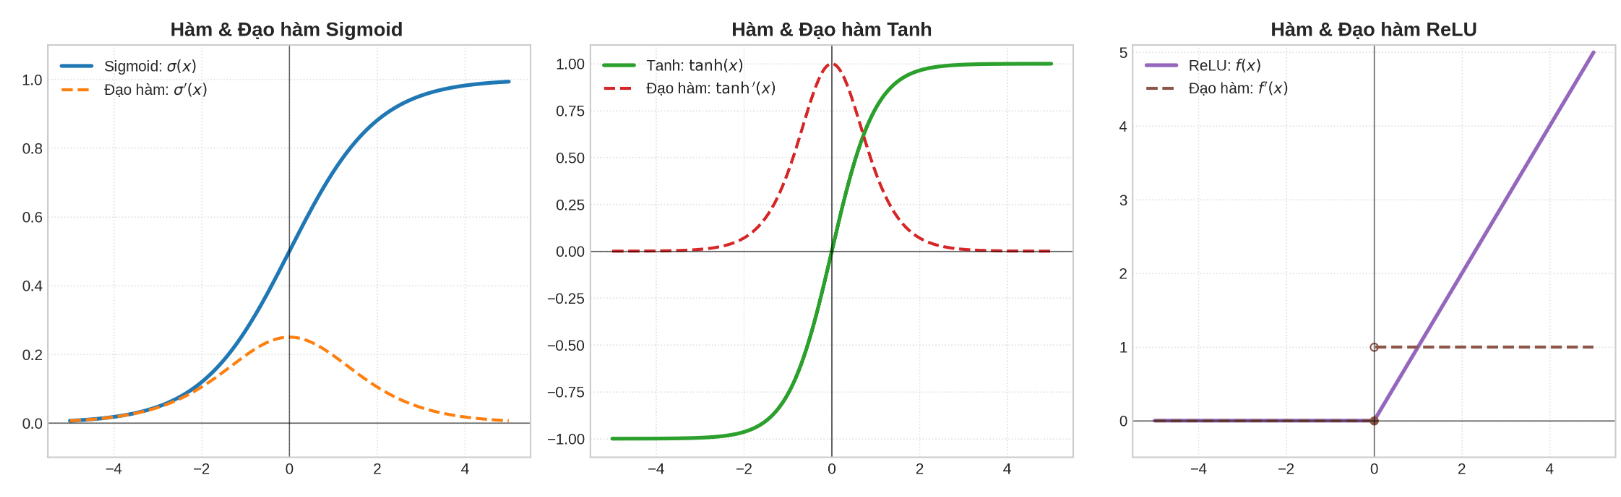
\includegraphics[width=\linewidth]{Images/04_Images/AFs.png}
    \caption{Các hàm kích hoạt Sigmoid, Tanh, ReLU và đạo hàm của chúng.}
\end{figure}

\begin{lstlisting}[caption={Mã Python cho các hàm kích hoạt ReLU, Sigmoid, Tanh và vẽ đồ thị hàm số cùng với đạo hàm của chúng.}, language=Python]
import numpy as np
import matplotlib.pyplot as plt

# 1. Dinh nghia ham kich hoat
def sigmoid(x):
    return 1 / (1 + np.exp(-x))

def sigmoid_derivative(x):
    s = sigmoid(x)
    return s * (1 - s)

def tanh(x):
    return np.tanh(x)

def tanh_derivative(x):
    return 1 - np.tanh(x)**2

def relu(x):
    return np.maximum(0, x)

# 2. Tao du lieu
x = np.linspace(-5, 5, 500)
x_neg = np.linspace(-5, 0, 250, endpoint=False) # x < 0
x_pos = np.linspace(0, 5, 250)[1:]              # x > 0

# 3. Ve do thi
fig, axes = plt.subplots(1, 3, figsize=(15, 4.5), dpi=300)

# --- Sigmoid ---
axes[0].plot(x, sigmoid(x), label=r'Sigmoid: $\sigma(x)$', color='#1f77b4', linewidth=2.5)
axes[0].plot(x, sigmoid_derivative(x), label=r"Dao ham: $\sigma'(x)$", color='#ff7f0e', linestyle='--', linewidth=2)
axes[0].set_title('Ham & Dao ham Sigmoid', fontsize=13, fontweight='bold')
axes[0].axhline(0, color='black', linewidth=0.8, alpha=0.6)
axes[0].axvline(0, color='black', linewidth=0.8, alpha=0.6)
axes[0].set_ylim(-0.1, 1.1)
axes[0].legend(loc='upper left')
axes[0].grid(True, linestyle=':', alpha=0.6)

# --- Tanh ---
axes[1].plot(x, tanh(x), label=r'Tanh: $\tanh(x)$', color='#2ca02c', linewidth=2.5)
axes[1].plot(x, tanh_derivative(x), label=r"Dao ham: $\tanh'(x)$", color='#d62728', linestyle='--', linewidth=2)
axes[1].set_title('Ham & Dao ham Tanh', fontsize=13, fontweight='bold')
axes[1].axhline(0, color='black', linewidth=0.8, alpha=0.6)
axes[1].axvline(0, color='black', linewidth=0.8, alpha=0.6)
axes[1].set_ylim(-1.1, 1.1)
axes[1].legend(loc='upper left')
axes[1].grid(True, linestyle=':', alpha=0.6)

# --- ReLU ---
axes[2].plot(x, relu(x), label=r'ReLU: $f(x)$', color='#9467bd', linewidth=2.5)
axes[2].plot(x_neg, np.zeros_like(x_neg), color='#8c564b', linestyle='--', linewidth=2, label=r"Dao ham: $f'(x)$")
axes[2].plot(x_pos, np.ones_like(x_pos), color='#8c564b', linestyle='--', linewidth=2)
axes[2].plot(0, 0, marker='o', markersize=5, color='#8c564b')
axes[2].plot(0, 1, marker='o', markersize=5, color='#8c564b', fillstyle='none')
axes[2].set_title('Ham & Dao ham ReLU', fontsize=13, fontweight='bold')
axes[2].axhline(0, color='black', linewidth=0.8, alpha=0.6)
axes[2].axvline(0, color='black', linewidth=0.8, alpha=0.6)
axes[2].set_ylim(-0.5, 5.1)
axes[2].legend(loc='upper left')
axes[2].grid(True, linestyle=':', alpha=0.6)

plt.tight_layout()
plt.savefig('activation_functions_thesis.png', dpi=300)
plt.show()
\end{lstlisting}























% \subsubsection{Sự suy biến của mạng nơ-ron tuyến tính đa tầng}

% \begin{definition}{Hàm kích hoạt đồng nhất\\}
% Toán tử kích hoạt đồng nhất $\sigma_{\mathrm{id}}: \mathbb{R} \to \mathbb{R}$ được xác định bởi ánh xạ đồng nhất trên trường số thực:
% \begin{equation}
%     \sigma_{\mathrm{id}}(z) = z, \qquad \forall z \in \mathbb{R}.
% \end{equation}
% Xét trên không gian vector đa chiều $\mathbf{z} \in \mathbb{R}^d$, toán tử vector $\boldsymbol{\sigma}_{\mathrm{id}}: \mathbb{R}^d \to \mathbb{R}^d$ tác động theo từng tọa độ chính là toán tử đồng nhất $\operatorname{id}_{\mathbb{R}^d}$, với tập ảnh: $\operatorname{Im}(\sigma_{\mathrm{id}}) = \mathbb{R}$.

% \textbf{Tính chất giải tích và đạo hàm.}
% \begin{enumerate}
%     \item \textit{Tính trơn:} Ánh xạ $\sigma_{\mathrm{id}}$ là một đẳng cấu tuyến tính và thuộc lớp hàm khả vi vô hạn $C^\infty(\mathbb{R})$.
%     \item \textit{Gradient bậc một:} Đạo hàm bậc nhất là một hằng số đơn vị trên toàn miền xác định:
%     \begin{equation}
%         \sigma_{\mathrm{id}}'(z) = 1, \qquad \forall z \in \mathbb{R}.
%     \end{equation}
%     Khi đó, ma trận Jacobian của phép biến đổi tọa độ đồng nhất là ma trận đơn vị: $\mathbf{J}_{\boldsymbol{\sigma}_{\mathrm{id}}}(\mathbf{z}) = \mathbf{I}_d$.
%     \item \textit{Sự triệt tiêu đạo hàm bậc cao:} Mọi đạo hàm cấp $k \ge 2$ đều đồng nhất bằng $0$:
%     \begin{equation}
%         \sigma_{\mathrm{id}}^{(k)}(z) = 0, \qquad \forall z \in \mathbb{R}, \quad \forall k \ge 2.
%     \end{equation}
% \end{enumerate}
% \end{definition}


% Xét một mạng nơ-ron truyền thẳng gồm $L$ lớp ẩn.
% Ký hiệu số lượng nơ-ron tại các lớp lần lượt là $n_0, n_1, \dots, n_{L+1}$, với $n_0 = d$ là số chiều đầu vào và $n_{L+1} = m$ là số chiều đầu ra.

% Tại mỗi lớp $l \in \{1, 2, \dots, L+1\}$, ma trận trọng số và véc-tơ độ lệch tương ứng được ký hiệu là $\mathbf{W}^{(l)} \in \mathbb{R}^{n_l \times n_{l-1}}$ và $\mathbf{b}^{(l)} \in \mathbb{R}^{n_l}$. Phép biến đổi affin ánh xạ từ véc-tơ kích hoạt của lớp trước $\mathbf{a}^{(l-1)}$ sang véc-tơ tiền kích hoạt của lớp hiện tại $\mathbf{z}^{(l)}$ được định nghĩa là:

% \begin{equation}
%     \mathbf{z}^{(l)} = T_l(\mathbf{a}^{(l-1)}) \triangleq \mathbf{W}^{(l)} \mathbf{a}^{(l-1)} + \mathbf{b}^{(l)},
% \end{equation}

% với quy ước $\mathbf{a}^{(0)} = \mathbf{x} \in \mathbb{R}^d$ là véc-tơ dữ liệu đầu vào. Tại mỗi lớp, véc-tơ kích hoạt đầu ra được tính bởi $\mathbf{a}^{(l)} = \sigma(\mathbf{z}^{(l)})$.

% \begin{theorem}{Sự suy biến của mạng nơ-ron tuyến tính đa tầng} \label{thm:linear_collapse}


% Giả sử tất cả $L+1$ lớp của mạng đều sử dụng hàm kích hoạt đồng nhất $\sigma_{\mathrm{id}}(z) = z$. Khi đó, hàm biểu diễn toàn cục của mạng $f: \mathbb{R}^d \to \mathbb{R}^m$ suy biến thành một phép biến đổi affine đơn tầng duy nhất:

% \begin{equation}
%     \mathbf{y} = f(\mathbf{x}) = \overline{\mathbf{W}}\mathbf{x} + \overline{\mathbf{b}}, \label{eq:collapsed_model}
% \end{equation}

% trong đó ma trận trọng số tổng hợp $\overline{\mathbf{W}} \in \mathbb{R}^{m \times d}$ và véc-tơ độ lệch tổng hợp $\overline{\mathbf{b}} \in \mathbb{R}^m$ được xác định tường minh bởi:

% \begin{align}
%     \overline{\mathbf{W}} &= \prod_{l=L+1}^{1} \mathbf{W}^{(l)} = \mathbf{W}^{(L+1)} \mathbf{W}^{(L)} \cdots \mathbf{W}^{(1)}, \label{eq:W_bar} \\
%     \overline{\mathbf{b}} &= \mathbf{b}^{(L+1)} + \sum_{i=1}^L \left( \prod_{j=L+1}^{i+1} \mathbf{W}^{(j)} \right) \mathbf{b}^{(i)}, \label{eq:b_bar}
% \end{align}

% với quy ước tích có thứ tự của các ma trận $\prod_{j=p}^{q} \mathbf{A}_j \triangleq \mathbf{A}_p \mathbf{A}_{p-1} \cdots \mathbf{A}_q$ khi $p \ge q$.
% \end{theorem}

% \begin{proof}
% Chúng ta sẽ chứng minh định lý bằng phương pháp quy nạp toán học theo số lớp $l$. Gọi $\mathbf{a}^{(l)}$ là véc-tơ đầu ra của lớp thứ $l$. Ta cần chứng minh:
% \begin{equation}
%     \mathbf{a}^{(l)} = \left( \prod_{j=l}^{1} \mathbf{W}^{(j)} \right) \mathbf{x} + \mathbf{b}^{(l)} + \sum_{i=1}^{l-1} \left( \prod_{j=l}^{i+1} \mathbf{W}^{(j)} \right) \mathbf{b}^{(i)}.
% \end{equation}

% \textbf{Cơ sở quy nạp ($l = 1$):} \\
% Do hàm kích hoạt là hàm đồng nhất, ta có:
% \begin{equation}
%     \mathbf{a}^{(1)} = \sigma_{\mathrm{id}}(\mathbf{z}^{(1)}) = \mathbf{W}^{(1)}\mathbf{a}^{(0)} + \mathbf{b}^{(1)} = \mathbf{W}^{(1)}\mathbf{x} + \mathbf{b}^{(1)}.
% \end{equation}
% Công thức đúng với $l = 1$ (tổng sigma bằng 0 theo quy ước tổng rỗng).

% \textbf{Bước quy nạp:} \\
% Giả sử công thức đúng cho lớp thứ $l = k$ ($1 \le k \le L$). Xét tại lớp thứ $k+1$:
% \begin{align*}
%     \mathbf{a}^{(k+1)} &= \sigma_{\mathrm{id}}(\mathbf{W}^{(k+1)}\mathbf{a}^{(k)} + \mathbf{b}^{(k+1)}) \\
%     &= \mathbf{W}^{(k+1)} \left[ \left( \prod_{j=k}^{1} \mathbf{W}^{(j)} \right) \mathbf{x} + \mathbf{b}^{(k)} + \sum_{i=1}^{k-1} \left( \prod_{j=k}^{i+1} \mathbf{W}^{(j)} \right) \mathbf{b}^{(i)} \right] + \mathbf{b}^{(k+1)} \\
%     &= \left( \mathbf{W}^{(k+1)} \prod_{j=k}^{1} \mathbf{W}^{(j)} \right) \mathbf{x} + \mathbf{W}^{(k+1)}\mathbf{b}^{(k)} + \sum_{i=1}^{k-1} \left( \mathbf{W}^{(k+1)} \prod_{j=k}^{i+1} \mathbf{W}^{(j)} \right) \mathbf{b}^{(i)} + \mathbf{b}^{(k+1)} \\
%     &= \left( \prod_{j=k+1}^{1} \mathbf{W}^{(j)} \right) \mathbf{x} + \mathbf{b}^{(k+1)} + \sum_{i=1}^{k} \left( \prod_{j=k+1}^{i+1} \mathbf{W}^{(j)} \right) \mathbf{b}^{(i)}.
% \end{align*}
% Theo nguyên lý quy nạp, công thức đúng với mọi $l \in \{1, \dots, L+1\}$. 
% Thay $l = L+1$ và đặt $\mathbf{y} = \mathbf{a}^{(L+1)}$, ta thu được chính xác kết quả của các phương trình \eqref{eq:W_bar} và \eqref{eq:b_bar}.
% \end{proof}


% \begin{proof}

% Vì $\sigma_{\mathrm{id}}$ là ánh xạ đồng nhất, vector kích hoạt tại mỗi tầng $l \in \{1, \dots, L+1\}$ thỏa $\mathbf{a}^{(l)} = \sigma_{\mathrm{id}}(\mathbf{z}^{(l)}) = \mathbf{z}^{(l)}$. Do đó, toàn bộ mạng tương đương với phép hợp thành liên tiếp của $L+1$ ánh xạ affine:

% \begin{equation}
%     \mathbf{y} = \mathbf{a}^{(L+1)} = (T_{L+1} \circ T_L \circ \dots \circ T_1)(\mathbf{x}).
% \end{equation}

% \textbf{Trường hợp 1: Mô hình thuần nhất không có độ lệch ($\mathbf{b}^{(l)} = \mathbf{0}, \forall l$).} \\
% Ta tiến hành chứng minh bằng quy nạp toán học theo số lớp $l$. 
% \begin{itemize}
%     \item \textit{Cơ sở quy nạp ($l = 1$):} $\mathbf{a}^{(1)} = \mathbf{W}^{(1)}\mathbf{x}$, mệnh đề hiển nhiên đúng.
%     \item \textit{Bước quy nạp:} Giả sử mệnh đề đúng đến lớp $p \le L$, nghĩa là:
%     \begin{equation}
%         \mathbf{a}^{(p)} = \left(\mathbf{W}^{(p)} \mathbf{W}^{(p-1)} \cdots \mathbf{W}^{(1)}\right) \mathbf{x}.
%     \end{equation}
%     Xét lớp $p+1$, theo tính kết hợp của phép nhân ma trận:
%     \begin{align}
%         \mathbf{a}^{(p+1)} &= \mathbf{W}^{(p+1)} \mathbf{a}^{(p)} \nonumber \\
%         &= \mathbf{W}^{(p+1)} \left[ \left(\mathbf{W}^{(p)} \mathbf{W}^{(p-1)} \cdots \mathbf{W}^{(1)}\right) \mathbf{x} \right] \nonumber \\
%         &= \left(\mathbf{W}^{(p+1)} \mathbf{W}^{(p)} \cdots \mathbf{W}^{(1)}\right) \mathbf{x}.
%     \end{align}
% \end{itemize}
% Theo nguyên lý quy nạp, tại lớp đầu ra $l = L+1$:
% \begin{equation}
%     \mathbf{y} = \mathbf{a}^{(L+1)} = \left(\prod_{j=L+1}^{1} \mathbf{W}^{(j)}\right) \mathbf{x} = \overline{\mathbf{W}}\mathbf{x}.
% \end{equation}

% \textbf{Trường hợp 2: Mô hình tổng quát có độ lệch ($\mathbf{b}^{(l)} \neq \mathbf{0}$).} \\
% Ta chứng minh công thức tổng quát của vector kích hoạt tại lớp  $k \in \{1, \dots, L+1\}$ bằng quy nạp:
% \begin{equation}
%     \mathbf{a}^{(k)} = \left( \prod_{j=k}^1 \mathbf{W}^{(j)} \right) \mathbf{x} + \mathbf{b}^{(k)} + \sum_{i=1}^{k-1} \left( \prod_{j=k}^{i+1} \mathbf{W}^{(j)} \right) \mathbf{b}^{(i)}. \tag{$*$}
% \end{equation}
% \begin{itemize}
%     \item \textit{Cơ sở quy nạp ($k = 1$):} 
%     $\mathbf{a}^{(1)} = \mathbf{W}^{(1)}\mathbf{x} + \mathbf{b}^{(1)}$. ($*$) đúng (tổng rỗng quy ước bằng $\mathbf{0}$).
%     \item \textit{Bước quy nạp:} Giả sử ($*$) đúng với $k = p \le L$. Tại lớp $p+1$:
%     \begin{align}
%         \mathbf{a}^{(p+1)} &= \mathbf{W}^{(p+1)} \mathbf{a}^{(p)} + \mathbf{b}^{(p+1)} \nonumber \\
%         &= \mathbf{W}^{(p+1)} \left[ \left( \prod_{j=p}^1 \mathbf{W}^{(j)} \right) \mathbf{x} + \mathbf{b}^{(p)} + \sum_{i=1}^{p-1} \left( \prod_{j=p}^{i+1} \mathbf{W}^{(j)} \right) \mathbf{b}^{(i)} \right] + \mathbf{b}^{(p+1)} \nonumber \\
%         &= \left( \mathbf{W}^{(p+1)} \prod_{j=p}^1 \mathbf{W}^{(j)} \right) \mathbf{x} + \mathbf{b}^{(p+1)} + \mathbf{W}^{(p+1)}\mathbf{b}^{(p)} + \sum_{i=1}^{p-1} \left( \mathbf{W}^{(p+1)} \prod_{j=p}^{i+1} \mathbf{W}^{(j)} \right) \mathbf{b}^{(i)} \nonumber \\
%         &= \left( \prod_{j=p+1}^1 \mathbf{W}^{(j)} \right) \mathbf{x} + \mathbf{b}^{(p+1)} + \sum_{i=1}^p \left( \prod_{j=p+1}^{i+1} \mathbf{W}^{(j)} \right) \mathbf{b}^{(i)}.
%     \end{align}
% \end{itemize}
% Như vậy, công thức ($*$) đúng với $k = p+1$. Đặt $k = L+1$, ta thu được chính xác biểu thức \eqref{eq:collapsed_model} với $\overline{\mathbf{W}}$ và $\overline{\mathbf{b}}$ cho bởi \eqref{eq:W_bar} và \eqref{eq:b_bar}. 
% \end{proof}

% % Từ Định lý \ref{thm:linear_collapse}, chúng ta có thể rút ra các tính chất đại số nền tảng và giới hạn nghiêm ngặt về dung lượng biểu diễn của các kiến trúc mạng không có hàm kích hoạt phi tuyến.

% \begin{remark}{Tính khép kín của phép hợp thành affine}

% Trong không gian các ánh xạ affine, phép toán hàm hợp có tính khép kín. Cụ thể, nếu $T_1: \mathbb{R}^p \to \mathbb{R}^q$ và $T_2: \mathbb{R}^q \to \mathbb{R}^r$ là các biến đổi affin, thì ánh xạ hợp thành $T_2 \circ T_1: \mathbb{R}^p \to \mathbb{R}^r$ cũng là một biến đổi affine. 
% Bản chất của Định lý \ref{thm:linear_collapse} chính là hệ quả của tính chất đại số cơ bản này khi áp dụng liên tiếp trên $L+1$ lớp.
% \end{remark}

% Kết quả này cho thấy việc tăng độ sâu của mạng không đem lại bất kỳ khả năng nội suy nào phức tạp hơn cho mô hình tuyến tính truyền thống. 

% % Thậm chí, khi kết hợp với cấu trúc phân loại ở lớp cuối, mạng suy biến về cấu trúc tối giản nhất:

% % \begin{corollary}{Sự suy biến về mô hình Perceptron đơn tầng}
% % \label{cor:perceptron_collapse}

% % Xét một mạng nơ-ron đa tầng với hàm kích hoạt đồng nhất tại tất cả các tầng ẩn. Tầng đầu ra gồm một nơ-ron duy nhất sử dụng hàm kích hoạt dấu $\mathrm{sgn}(\cdot)$ để thực hiện bài toán phân loại nhị phân. Giá trị dự đoán được tính bởi:
% % \begin{equation}
% %     \hat{y} = \mathrm{sgn}\left(\mathbf{w}^{(L+1)\top} \mathbf{a}^{(L)} + b^{(L+1)}\right).
% % \end{equation}
% % Khi đó, toàn bộ kiến trúc mạng biểu diễn chính xác một mô hình Perceptron đơn tầng (Rosenblatt Perceptron):
% % \begin{equation}
% %     \hat{y} = \mathrm{sgn}\left(\overline{\mathbf{w}}^\top \mathbf{x} + \overline{b}\right),
% % \end{equation}
% % trong đó vector trọng số tổng hợp $\overline{\mathbf{w}}^\top = \mathbf{w}^{(L+1)\top} \prod_{j=L}^1 \mathbf{W}^{(j)} \in \mathbb{R}^{1 \times d}$ và $\overline{b} \in \mathbb{R}$ được tính theo phương trình \eqref{eq:b_bar}.
% % \end{corollary}

% % Nghiêm trọng hơn việc không thể học được các mặt phân định phi tuyến, mạng nơ-ron tuyến tính đa tầng còn phải đối mặt với hiện tượng mất mát thông tin không thể phục hồi do cấu trúc hạng của ma trận.

% % \begin{corollary}{Giới hạn dung lượng biểu diễn do hiện tượng thắt nút cổ chai}

% % \label{cor:rank_bottleneck}
% % Giả sử bỏ qua các vector độ lệch $\mathbf{b}$ để đơn giản hóa, phép biến đổi tổng hợp của mạng là $\mathbf{y} = \overline{\mathbf{W}}\mathbf{x}$. Theo tính chất của hạng ma trận đối với phép nhân, ta luôn có:
% % \begin{equation}
% %     \mathrm{rank}(\overline{\mathbf{W}}) = \mathrm{rank}\left(\prod_{l=L+1}^1 \mathbf{W}^{(l)}\right) \le \min_{1 \le l \le L+1} \{ \mathrm{rank}(\mathbf{W}^{(l)}) \} \le \min_{0 \le l \le L+1} \{n_l\}. \label{eq:rank_bottleneck}
% % \end{equation}
% % \end{corollary}

% % Phương trình \eqref{eq:rank_bottleneck} chỉ ra một giới hạn cứng: Nếu tồn tại bất kỳ tầng ẩn $l$ nào có số lượng nơ-ron $n_l < \min(d, m)$, ma trận tham số tổng hợp $\overline{\mathbf{W}}$ sẽ trở thành ma trận suy biến. Cấu trúc này tạo ra một \emph{nút thắt cổ chai thông tin}, ép toàn bộ dữ liệu đầu vào phải chiếu qua một không gian con affin có số chiều nhỏ hơn, dẫn đến sự phá hủy thông tin không thể đảo ngược. Trái lại, khi sử dụng các hàm kích hoạt phi tuyến $\sigma$ (như ReLU, Tanh), mạng nơ-ron có thể phá vỡ ràng buộc về không gian con tuyến tính này, bảo toàn thông tin chiều cao và ánh xạ dữ liệu lên các đa tạp phi tuyến phức tạp.


